% !TeX root = S6_IntNum_TP_Bloc_VI_TP1_2_Banc_OpenCV.tex
%%%%%%%%%%%%%%%%%%%%%%%%%%%%%%%%%%%%%%%%%%
% Engineering problems / LaTeX Template
%		Semester 6
%		Institut d'Optique Graduate School
%%%%%%%%%%%%%%%%%%%%%%%%%%%%%%%%%%%%%%%%%%
%	6N-IntNum-BlocVI
%%%%%%%%%%%%%%%%%%%%%%%%%%%%%%%%%%%%%%%%%%
%
% Created by:
%	Julien VILLEMEJANE - 20/nov/2025
%	
%
%%%%%%%%%%%%%%%%%%%%%%%%%%%%%%%%%%%%%%%%%%


%%%%%%%%%%%%%%%%%%%%%%%%%%%%%%%%%%%%%%%%%%%%%%%%
%%%%%%%%%%%%%%%%%%%%%%%%%%%%%%%%%%%%%%%%%%%%%%%%
%%  TP 1


\newpage
\begin{center}
	\begin{minipage}{2.5cm}
	\begin{center}
		
\includegraphics[width=5cm]{../images/Logo-LEnsE.png}
	\end{center}
\end{minipage}\hfill
\begin{minipage}{10cm}
	\begin{center}
	\textbf{Institut d'Optique Graduate School }\\[0.1cm]
    \textbf{Interfaçage Numérique}


	\end{center}
\end{minipage}\hfill


\vspace{2cm}


{\Large \bfseries \textsc{Interfaçage Numérique}} \\[0.5cm]
{\large \bfseries Travaux Pratiques} \\[0.2cm]
Semestre 6

\vspace{1cm}

% Title
\rule{\linewidth}{0.4mm} \\[0.4cm]
{ \Large \bfseries\color{violet_iogs} TP1 - Banc de vision industrielle \\[0.4cm] }
\rule{\linewidth}{0.4mm} \\[1cm]

\end{center}

\vfill


\bigskip

\textbf{Une feuille de résultats est à remplir et à présenter tout au long de la séance de TP.}


%%%%%%%%%%%%%%%%%%%%%%%%%%%%%%%%%%%%%%%%%%%%%%%%
%%%%%%%%%%%%%    A A V / Objectifs

\section{Chaîne de vision industrielle}

Cette séance se base sur un \textbf{banc de vision industrielle} contenant un éclairage annulaire, une caméra et son objectif, des objets à analyser et d'un logiciel de pilotage de la caméra.

\medskip

Cette séance a pour but :
\begin{itemize}
	\item d'\textbf{analyser l'impact des différents maillons} d'une chaîne d'acquisition sur la qualité de l'image
	\item de \textbf{proposer des méthodes quantitatives de mesure} de la qualité d'image
	\item de \textbf{modéliser cette chaine} de manière simple
\end{itemize} 

\begin{center}
	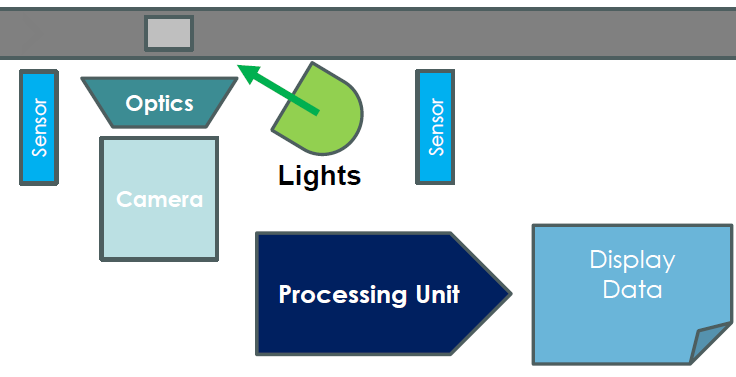
\includegraphics[width=0.5\textwidth]{../images/vi_chaine.png}
\end{center}

\textit{Ce document est complété par un \textbf{diaporama présentant quelques notions de base de la vision industrielle} / Disponible sur le site du LEnsE ou dans le document de ressources.}


\newpage
%%%%%%%%%%%%%%%%%%%%%%%%%%%%%%%%%%%%%%%%%%%%%%%%
%%%%%%%%%%%%%    Etape par étape

\section{A - Prise en main de l'interface {[30 min]}}

\Manip Allumer l'\textbf{éclairage annulaire} du banc (trois couleurs). Placer un \textbf{fond uniforme} sous l'éclairage (feuille blanche, paillasse...).

\Quest Quelle couleur d'éclairage obtient-on ?

\Manip Lancer l'application depuis \fbox{\textsc{S:/\_gui/Start\_VI.bat}}.

\noindent \rule{\linewidth}{1pt}

\Manip Ouvrir l'onglet \fbox{\textsc{Image ou Caméra}}.

\textit{Si la caméra est bien connectée en USB à l'ordinateur, vous devriez voir s'afficher son flux.}

\Manip Ouvrir l'onglet \fbox{\textsc{Zone d'intérêt}}. 

\textit{Cet onglet servira par la suite à définir une zone d'acquisition plus restreinte.}

\subsection{Histogramme}

\Manip Ouvrir l'onglet \fbox{\textsc{Histogramme}} puis sélectionner le mode \fbox{\textsc{Répartition spatiale}}.

\medskip

Dans cette section, vous allez pouvoir :

\begin{itemize}
	\item visualiser l'histogramme de l'image acquise par la caméra, le sauvegarder
	\item sauvegarder l'image acquise
	\item modifier le temps d'exposition et le black level de la caméra
\end{itemize}

\medskip

\Quest Que représente l'histogramme d'une image ? A quoi peut-il servir ?

\Manip Placer le \textit{black level} à 0. Modifier le \textbf{temps d'intégration} de la caméra. 

\Quest Que se passe-t-il sur l'image ? Sur l'histogramme ?

\Quest Quelles sont les valeurs minimale et maximale que peuvent prendre les pixels de la caméra ? Quelle est alors la \textbf{profondeur binaire} de la caméra utilisée ?

\noindent \rule{\linewidth}{1pt}

L'objectif monté sur la caméra possède 2 bagues qui permettent de changer : l'\textbf{ouverture numérique de l'objectif} et la \textbf{mise au point}.

\Manip Imposer un temps d'intégration qui ne sature pas le capteur (pour un éclairage blanc). Modifier l'ouverture numérique d'un cran. 

\Quest Que se passe-t-il sur l'image ? Sur l'histogramme ?


\subsection{Mise au point et zone d'intérêt}

\Manip Placer la mire graduée (zone avec écriture) dans le champ de la caméra. Ajuster la seconde bague de l'objectif pour faire la mise au point sur l'objet.

\Manip Dans l'onglet \fbox{\textsc{Zone d'intérêt}}, ajuster la zone d'intérêt (ou \textit{Area of Interest} - AOI) pour ne sélectionner qu'une partie de l'image autour de l'objet (environ 500 pixels par 500 pixels).

\noindent \rule{\linewidth}{1pt}

\textit{\textbf{Pour la suite du TP, on s'assurera de prendre une zone d'intérêt à peu près centrée dans l'image et d'une taille d'environ 500 par 500 pixels.}}

\noindent \rule{\linewidth}{1pt}

\subsection{Profil dans l'image}

\Manip Placer des cubes de couleur dans le champ de la caméra. Sélectionner une zone d'intérêt d'environ 500 pixels par 500 pixels autour des objets à visualiser. Ajuster le temps d'intégration pour obtenir une image non saturée avec un éclairage blanc. 

\Quest Commenter l'image et l'histogramme obtenus. Que se passe-t-il avec un cube d'une autre couleur ?

\Manip Ouvrir l'onglet \fbox{\textsc{Outils pour Images}} puis sélectionner le mode \fbox{\textsc{Profil dans l'image}}.

\Manip Déplacer les positions des profils horizontal et vertical. Observer les profils obtenus pour différentes positions.

\Quest Quel est l'intérêt d'un tel outil ?


\subsection{Echantillonnage et quantification}

\textit{Conserver les objets dans le champ de la caméra.}

\Manip Ouvrir l'onglet \fbox{\textsc{Quantif./Echant.}} puis sélectionner le mode \fbox{\textsc{Impact de la quantification}}.

\Manip Modifier la profondeur de gris et visualiser l'effet sur l'image et sur l'histogramme après traitement.

\Quest Que peut-on conclure sur l'effet de la quantification sur l'image ?

\noindent \rule{\linewidth}{1pt}

\Manip De la même façon, avec le mode \fbox{\textsc{Impact de l'échantillonnage}}, modifier le nombre de pixels de sous-échantillonnage. 

On parle ici d'un phénomène de \textbf{binning}. La résolution de l'image est "dégradée" numériquement dans ce cas et les nouveaux pixels affichés sont la moyenne de N x N pixels de l'image initiale.

\textit{Dans le cas présent, ce phénomène peut simuler le changement de résolution de la caméra sur l'acquisition d'une image numérique.}

\Quest Que peut-on conclure sur l'effet de la résolution de la caméra sur l'image ?


\section{B - Outils numériques de base {[30 min]}}

Dans cette section, nous allons nous intéresser à quelques fonctionnalités permettant de \textbf{manipuler des images} pour les rendre utilisables : amélioration du contraste, seuillage, suppression du bruit...

\subsection{Contraste et Luminosité}

\Manip Placer un cube de couleur dans le champ de la caméra. Sélectionner une zone d'intérêt d'environ 500 pixels par 500 pixels autour de l'objet à visualiser. Ajuster le temps d'intégration pour obtenir un histogramme dont le pixel maximum a une valeur de l'ordre des 2/3 de la valeur maximale de la caméra. 

\Manip Ouvrir l'onglet \fbox{\textsc{Pré-Traitement}} puis sélectionner le mode \fbox{\textsc{Contraste / Luminosité}}.

\Manip Modifier les valeurs de contraste et de luminosité de l'image.

\Quest Quelles sont les opérations mathématiques réalisées sur les pixels par ces deux fonctionnalités ? Vous pourrez vous appuyer sur les histogrammes des images brutes et modifiées pour analyser vos résultats.

\Manip Avec le mode \fbox{\textsc{Amélioration du Contraste}}, tester l'effet des deux curseurs.

\Quest Proposer une interprétation de l'opération effectuée sur chacun des pixels.


\subsection{Seuillage}

\Manip Ouvrir l'onglet \fbox{\textsc{Pré-Traitement}} puis sélectionner le mode \fbox{\textsc{Seuillage}}.

\Manip Sélectionner le seuillage \textsl{Normal} et modifier la valeur du seuil.

\Quest Que pouvez-vous conclure sur l'intérêt du seuillage ? Vous pourrez essayer avec des objets de taille, de forme et de couleurs différentes.

\Manip Tester également le mode \textsl{Inversé} et \textsl{Double}.

\Quest Que pouvez-vous conclure sur ces deux modes ?
 

\subsection{Filtrage}

\Manip Ouvrir l'onglet \fbox{\textsc{Filtres}} puis sélectionner le mode \fbox{\textsc{Filtre de lissage}}.

\Manip Sélectionner le filtre \textsl{Blur Moyen} et un noyau de taille 15.

\Quest Que se passe-t-il sur l'image ? Vous pourrez également vous appuyer sur la différence entre l'image de base et l'image modifiée, en cliquant sur l'option \textsl{Image - Effet}, pour analyser les effets sur l'image.

\Quest Quel est l'effet de la taille du noyau sur le filtrage ?

\Quest Qu'en est-il avec les filtres de type \textsl{Blur Gaussien} et \textsl{Médian} ? 

\vfill

\textit{Les aspects théoriques liés au filtrage de données (signaux et images) sont abordés dans les modules \textsc{Maths et Signal} (semestre 5) et \textsc{Traitement du Signal} (semestre 6).}

\textit{La mise en oeuvre de ces filtres sur des images sera abordée en TD de ce module et également dans des modules de traitement d'images dans vos prochaines années de formation.}


\newpage
\section{C - Contrôle de l'uniformité de l'éclairage {[20 min]}}

L'\textbf{éclairage} joue un rôle central dans tout système de vision industrielle, car il conditionne directement la qualité des images et, par conséquent, la fiabilité des algorithmes d'inspection ou de détection. Un choix d'éclairage adapté permet de révéler les caractéristiques pertinentes d'une scène — contrastes, reliefs, défauts de surface, contours — tout en minimisant les reflets indésirables, les ombres ou le bruit visuel. 

Un choix raisonné de l'éclairage constitue un élément déterminant pour garantir la robustesse, la répétabilité et la précision du système de vision industrielle.

\subsection{Uniformité de l'éclairage EFFI-Ring}

Nous allons nous intéresser ici à l'éclairage \textbf{Effilux EFFI-Ring}, version RGB et en particulier à l'uniformité de celui-ci en fonction de la distance de travail.

\textit{Quelques données sur cette source sont fournies en annexe de ce document.}

\Manip Allumer l'\textbf{éclairage annulaire} du banc (trois couleurs). Placer un \textbf{fond uniforme} sous l'éclairage (feuille blanche, paillasse...).

\Manip Sélectionner l'\textbf{ensemble du champ visible} par la caméra. Ajuster le temps d'intégration pour obtenir une image non saturée avec un éclairage blanc. Noter le temps d'intégration choisi. 

\Manip Ouvrir l'onglet \fbox{\textsc{Outils pour Images}} puis sélectionner le mode \fbox{\textsc{Profil dans l'image}}. Visualiser les profils vertical et horizontal au centre de l'image (environ).

% A terme ! Outil de mesure du profil (ou sauvegarde du profil pour analyse par la suite)

\Manip Mesurer les niveaux de gris minimal et maximal obtenus pour cet éclairement. 

\Quest Que pouvez-vous conclure sur l'éclairage à cette distance de travail ? 

\noindent \rule{\linewidth}{1pt}

On souhaite à présent remplir le tableau XX de la feuille de résultats et mesurer l'écart d'intensité relevé dans la zone centrale du champ de vision pour 3 hauteurs de travail différentes.

\Manip Sélectionner une zone d'intérêt de 400 x 400 pixels au centre du champ de vision de la caméra.

\Manip Mesurer les niveaux de gris minimal et maximal obtenus pour \textbf{3 hauteurs de travail différentes} : 25cm, 12cm et 6cm (environ) entre le fond et la caméra. 

\medskip

\textit{\textbf{Ne déplacer pas la potence de la caméra}. Déplacer un support uniforme sous la caméra (feuille blanche par exemple)}.

\medskip

\Quest Retrouve-t-on une courbe de réponse proche de celle du constructeur ?

\vfill

\subsection{Autres éclairages}

Selon la nature de la pièce à analyser (métallique, transparente, texturée...), de son mouvement et du type de défauts ou d'objets à détecter, différentes stratégies d'illumination (lumière rase, diffuse, coaxiale, structurée, stroboscopique...) peuvent être mises en oeuvre. 

\textit{Une démonstration est possible ! environ 10 min}


\newpage
\section{D - Linéarité du capteur {[30 min]}}

On souhaite vérifier la linéarité du capteur en fonction du temps d'intégration, pour les 3 couleurs d'éclairage ainsi que du blanc. On souhaite alors remplir le tableau XX de la feuille de résultats.

\Manip Placer un cube de couleur dans le champ de la caméra. Allumer l'éclairage annulaire en blanc. Ajuster la zone d'intérêt pour visualiser une zone quasiment uniforme de l'objet. Placer le \textit{black level} à 0.

\Manip Ajuster le temps d'intégration le plus élevé de vos relevés de mesure pour obtenir un histogramme dont les valeurs de niveau de gris ne dépassent les  2/3 de la valeur maximale de la caméra. 

\Quest Quel type de profil obtient-on ? Quelle forme d'histogramme ?

\Manip Pour différentes valeurs de temps d'intégration, relever (graphiquement) sur l'histogramme le niveau de gris du pic le plus élevé.

\Quest Quelle relation obtient-on entre ce niveau de gris et le temps d'intégration ? Que peut-on en conclure sur le capteur ?



\section{E - Champ de vision et résolution spatiale {[40 min]}}

Le \textbf{champ de vision} (\textit{field of view} en anglais) d'un système de vision (champ transversal à l'axe optique) correpond à l'ensemble des points de la scène imagée à travers le système optique (voir figure~\ref{fig:fov}). 

Il dépend de : 

\begin{itemize}
	\item la distance focale de l'objectif,
	\item de la taille du capteur de la caméra,
	\item de la distance de travail 
\end{itemize}

\medskip

Selon la dimension de la scène à visualiser, cette grandeur peut s'exprimer par des dimensions (scène à distance finie) ou par des angles (scène à distance infinie).

\begin{figure}[!h]
\begin{center}
	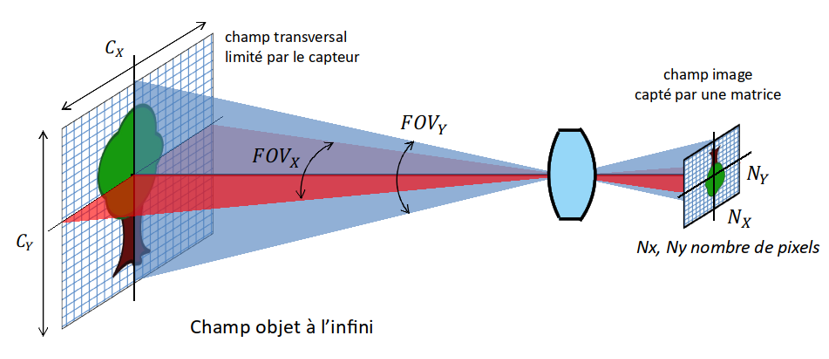
\includegraphics[width=0.8\textwidth]{../images/optique_champ_derossi.png}
	\caption{Système optique et champ de vision d'une caméra numérique - illustration provenant du cours d'optique instrumentale de Sébastien de Rossi.}
	\label{fig:fov}
\end{center}
\end{figure}

\medskip

\Manip Relever sur l'objectif sa focale.

\Manip Placer une règle graduée sur un fond uniforme dans le champ de la caméra.

\Manip Sélectionner l'ensemble du champ visible par la caméra. Ajuster le temps d'intégration pour obtenir une image non saturée avec un éclairage blanc. Faire la mise au point sur les graduations de la règle.

\Manip Mesurer le champ selon la hauteur ($C_Y$) et la largeur ($C_X$) de la scène.

\Quest A distance de travail équivalente, que devient le champ de vision pour un objectif de focale 2 fois plus courte ?

\noindent \rule{\linewidth}{1pt}

Quelques \textbf{données sur la caméra utilisée sont fournies en annexe} de ce document.

\Quest Quelle est la taille d'un pixel ? Quelle est la taille du capteur (hauteur - $N_Y$ - et largeur - $N_X$) en pixels ? Puis en mm ?

\Quest Rappeler les formules de conjugaison et de grandissement en optique instrumentale.

\Quest Calculer le grandissement obtenu avec le système optique lorsque l'on mesure un objet positionné sur le plan de travail (distance de travail fixée).

\Quest Vérifier par le calcul que la focale mentionnée sur l'objectif est correcte.

\noindent \rule{\linewidth}{1pt}

\Quest A partir des dimensions mesurées précédemment (champ de vision) et de la taille du capteur, qu'elle est la taille minimale qu'il est possible de mesurer à l'aide de ce système de vision ?

\Quest Que devient cette valeur si on rapproche l'objet de la caméra en divisant la hauteur de travail par 2 ? Le champ de vision est-il modifié ?

\medskip

Pour le vérifier, nous allons utiliser des mires de type Foucault. Ces mires sont des répétitions spatiales d'un même motif (succession de bandes noires et blanches) espacé d'une distance connue.

\Manip Placer une mire dans le champ de la caméra.

\Manip Ajuster la zone d'intérêt. Ajuster le temps d'intégration pour obtenir une image non saturée avec un éclairage blanc (maximum au 2/3 de l'histogramme). Faire la mise au point sur les graduations de la mire.

\Quest Quelle est la plus petite mire que vous arrivez à distinguer ?

\noindent \rule{\linewidth}{1pt}

\Manip Tracer le profil (horizontal ou vertical) passant par le centre des bandes de la mire.

\Quest Que constatez-vous en fonction du pas de la mire ?

\Manip Mesurer la hauteur des variations pour différents espacements des bandes.

\medskip

En normalisant ces mesures par rapport à la plus grande variation, on peut mesurer le contraste obtenu pour différentes fréquences spatiales de votre système de vision. On peut assimiler à la \textbf{fonction de transfert de modulation} (ou FTM). Cette donnée sert à caractériser les systèmes optiques en reliant la luminance de l'espace objet à l'éclairement de l'espace image. Cela permet de modéliser l'influence du système optique sur la distribution de l'énergie lumineuse dans l'espace image.

\medskip

\Manip Réduire le temps d'intégration et reprendre les mesures précédentes.

\Quest Le contraste est-il dépendant du temps d'intégration de la caméra ?

\noindent \rule{\linewidth}{1pt}

\Quest Comment peut-on mesurer des objets à partir d'une image numérique de celui-ci ?

\Manip Placer un cube de couleur dont vous aurez au préalable mesuré un des côtés. Tester la méthode proposée pour mesurer numériquement cet objet.

\Quest Quelle est la précision de la mesure ?

\newpage
\section{F - Première modélisation {[50 min]}}

Dans cette section, nous allons nous intéressé à la visualisation d'objets colorés par l'intermédiaire d'une caméra monochrome et de sources ayant des longueurs d'onde connues et distinctes, afin de donner un premier modèle simplifiée d'une chaine d'acquisition d'image (voir figure~\ref{fig:model}).

\begin{figure}[!h]
\begin{center}
	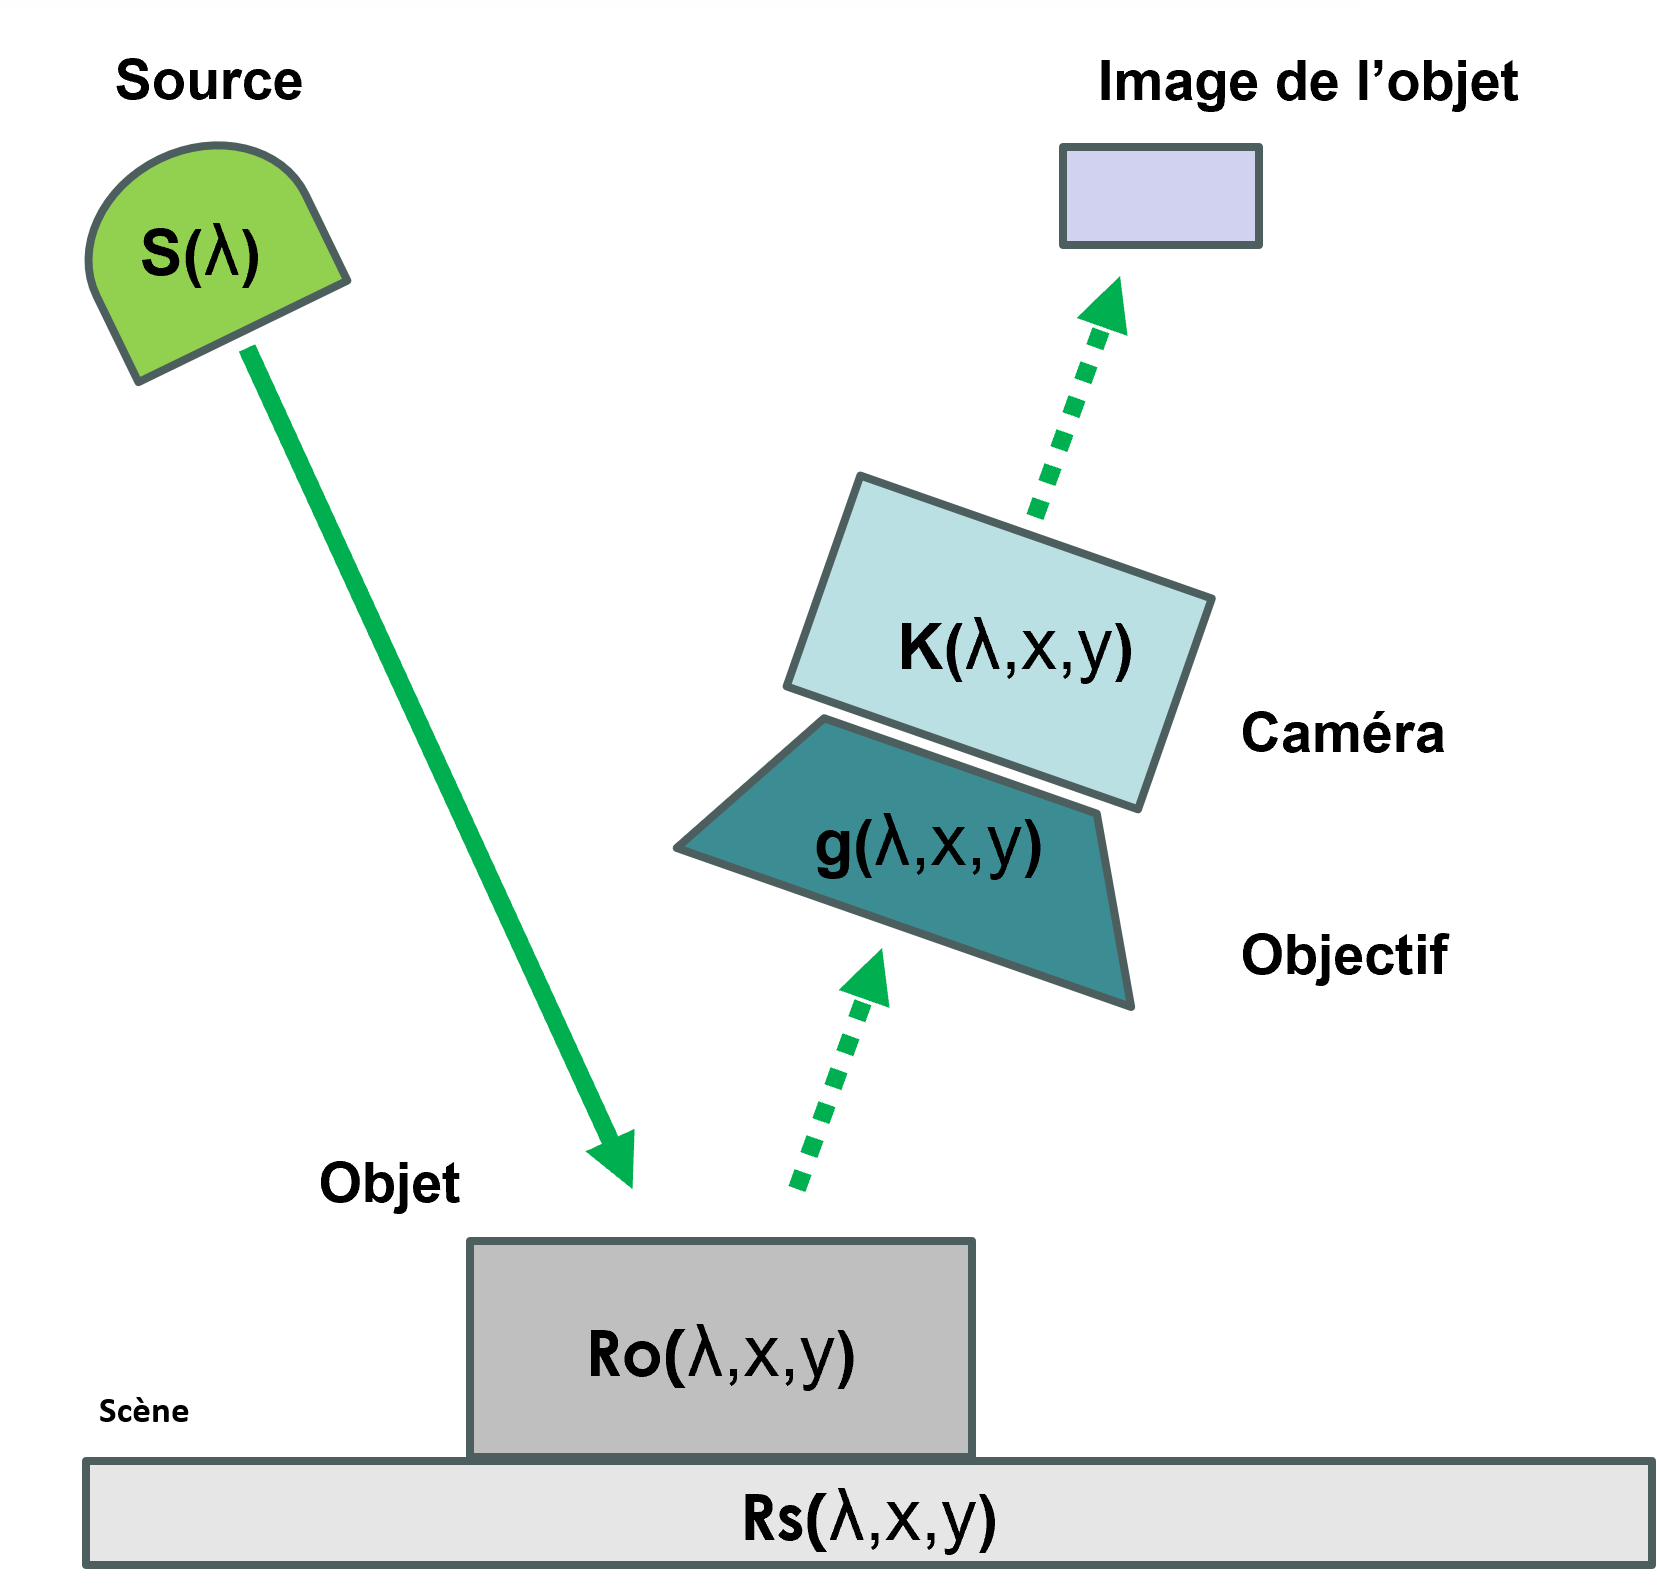
\includegraphics[width=0.55\textwidth]{../images/vi_model_chaine.png}
	\caption{Modélisation simplifiée d'une chaîne d'acquisition d'une image. $S(\lambda)$ : source primaire modélisée par son spectre en longueur d'onde ($\lambda$). $K(\lambda, x, y)$ : le gain de la caméra. $g(\lambda, x, y)$ le facteur de transmission de l'optique (en négligeant pour l'instant les aberrations). $R_0(\lambda, x, y)$ : réflectance de l'objet à visualiser. $R_S(\lambda, x, y)$ : réflectance des autres objets de la scène (en particulier le fond). }
	\label{fig:model}
\end{center}
\end{figure}

\medskip

On donne en annexe les réflectances des cubes de couleur que vous avez à votre disposition.

\medskip

\Quest En plaçant chacun des cubes de couleurs sous l'éclairage Rouge, lequel sera le plus "lumineux" ? 

\Quest Classer, théoriquement, les 4 cubes de couleur par ordre de luminosité pour les 3 éclairages disponibles.

\Quest Proposer alors une méthode de discrimination des cubes en fonction de leur couleur à l'aide du système de vision industrielle mis à votre disposition. \textbf{Cette méthode doit être robuste à un changement de temps d'intégration.}


\noindent \rule{\linewidth}{1pt}

\Manip Placer les cubes de couleur dans le champ de la caméra l'un après l'autre. Sélectionner une zone d'intérêt d'environ 500 pixels par 500 pixels autour des objets à visualiser. 

\Manip Pour chaque source (Rouge, Vert, Bleu) et pour chaque cube de couleur (pour un temps d'intégration donné et fixé pour l'ensemble des mesures), relever la valeur moyenne d'intensité lumineuse. 

\Quest Les résultats sont-ils cohérents avec la théorie ?

\Manip Mettre en oeuvre votre méthode de détection des couleurs et présenter vos résultats.


